\documentclass[12pt]{article}
\usepackage[left=1cm, right=1cm, top=2cm,bottom=1.5cm]{geometry} 

\usepackage[parfill]{parskip}
\usepackage[utf8]{inputenc}
\usepackage[T2A]{fontenc}
\usepackage[russian]{babel}
\usepackage{enumitem}
\usepackage[normalem]{ulem}
\usepackage{amsfonts, amsmath, amsthm, amssymb, mathtools}

\usepackage{fancyhdr}
\pagestyle{fancy}
\renewcommand{\headrulewidth}{1.5pt}
\renewcommand{\footrulewidth}{1pt}

\usepackage{graphicx}
\usepackage[figurename=Рис.]{caption}
\usepackage{subcaption}
\usepackage{float}

%%Наименование папки откуда забирать изображения
\graphicspath{ {./images/} }

%%Изменение формата для ввода доказательства
\renewcommand{\proofname}{$\square$  \nopunct}
\renewcommand\qedsymbol{$\blacksquare$}

\addto\captionsrussian{%
	\renewcommand{\proofname}{$\square$ \nopunct}%
}
%% Римские цифры
\newcommand{\RN}[1]{%
	\textup{\uppercase\expandafter{\romannumeral#1}}%
}


\theoremstyle{definition}
\newtheorem{defn}{Опр:}
\newtheorem{rem}{Rm:}
\newtheorem{prop}{Утв.}
\newtheorem{exrc}{Упр.}
\newtheorem{lemma}{Лемма}
\newtheorem{theorem}{Теорема}
\newtheorem{corollary}{Следствие}

\newenvironment{cusdefn}[1]
{\renewcommand\thedefn{#1}\defn}
{\enddefn}



\DeclareRobustCommand{\divby}{%
	\mathrel{\text{\vbox{\baselineskip.65ex\lineskiplimit0pt\hbox{.}\hbox{.}\hbox{.}}}}%
}


\newcommand{\smallerrel}[1]{\mathrel{\mathpalette\smallerrelaux{#1}}}
\newcommand{\smallerrelaux}[2]{\raisebox{.1ex}{\scalebox{.75}{$#1#2$}}}

\newcommand{\smallin}{\smallerrel{\in}}
\newcommand{\smallnotin}{\smallerrel{\notin}}



\begin{document}
	\lhead{Математический анализ - I}
	\chead{Шапошников С.В.}
	\rhead{Лекция - 9}

\section*{Подпоследовательности}

\begin{defn}
	Если задана последовательность $\{a_n\}$ и последовательность возрастающих номеров $n_1 < n_2 < n_3 < \dotsc < n_k < n_{k+1} < \dotsc$ - натуральные числа, то последовательность $\{a_{n_k}\}$ называется \uwave{подпоследовательностью} последовательности $\{a_n\}$.
\end{defn}

\subsection*{Примеры}

$a_n \colon 1, 2, 3, 1, 2, 3, 1, 2, 3, \dotsc$; $n_k = 2k \Rightarrow a_{n_k} \colon 2, 1, 3, \dotsc$ - подпоследовательность.\\ 
$n_1 = 2, a_{n_1} = 2; n_2 = 1, a_{n_2} = 1; \dotsc$ - не будет подпоследовательностью. 


$a_n \colon 1, 1, 1, 5, 5, 5, \dotsc$; $a_{n_k} \colon 5, 5, 1, 5, 5, \dotsc$ - не будет подпоследовательностью.

\begin{theorem}
	Если последовательность $a_n$ сходится к $a$, то всякая ее подпоследовательность $a_{n_k}$ будет сходится к $a$.
\end{theorem}
\begin{proof} Докажем сначала вспомогательное утверждение:
	\begin{enumerate}[label={(\arabic*)}]
		\item $n_k \geq k$ - по индукции: $k = 1$ - верно, так как $n_1$ - натуральное. Предположим, что для $k$ - верно, докажем для $k+1$: значем, что $n_{k+1} > n_k \geq k \Rightarrow$ так как числа - натуральные, то $n_{k+1} \geq n_k + 1 \geq k + 1$.
		\item Тогда по опр.: $\forall \varepsilon > 0,\, \exists \, N \colon \forall n > N,\, |a_n - a| < \varepsilon$. Пусть $k > N$, тогда $n_k \geq k > N \Rightarrow |a_{n_k}\! - a| < \varepsilon$.
	\end{enumerate}
\end{proof}

\begin{theorem}
	\textbf{(Больцано)}: Если последовательность $a_n$ - ограничена, то в ней есть сходящаяся подпоследовательность.
\end{theorem}
\begin{proof}
	\begin{figure}[H]
		\centering
		\includegraphics[width=0.45\textwidth]{9_1.eps}
		\caption{Идея доказательства}
		\label{9_1}
	\end{figure}

Пусть $a_n \in [\alpha_1, \beta_1 ]$, $l = \beta_1 - \alpha_1$ (так, как $a_n$ - ограниченно). Делим отрезок $[\alpha_1, \beta_1 ]$ пополам и берем в качестве отрезка $[\alpha_2, \beta_2]$ ту половину в которой бесконечно много членов последовательности $a_n$. Замечаем, что $\beta_2 - \alpha_2 = \dfrac{l}{2}$. Продолжая построение, получаем последовательность вложенных отрезков: $[\alpha_1, \beta_1] \supset [\alpha_2, \beta_2] \supset \dotsc \supset [\alpha_k, \beta_k] \supset \dotsc$ таких, что:

\begin{enumerate}[label={\arabic*)}]
	\item в каждом $[\alpha_k, \beta_k]$ бесконечно много членов последовательности $a_n$;
	\item $\beta_k - \alpha_k = \dfrac{l}{2^{k-1}} \xrightarrow[k \rightarrow \infty]{} 0$;
\end{enumerate}

$\forall k$ находим $a_{n_k} \in [\alpha_k, \beta_k]$ так, что $n_1 < n_2 < \dotsc$ - это возможно по 1)-ому свойству отрезков.

По теореме о вложенных отрезках существует $c \in \bigcap\limits_k [\alpha_k, \beta_k]$. Так как $a_{n_k} \in [\alpha_k, \beta_k]$ и $c \in [\alpha_k, \beta_k]$, то $|a_{n_k}\! - c| \leq \dfrac{l}{2^{k-1}} \rightarrow 0$, то есть $a_{n_k} \rightarrow c$.
\end{proof}

\begin{defn}
	Предел подпоследовательности называется \uwave{частичным пределом}.
\end{defn}

\uline{Задача}: описать множество частичных подпределов.

\begin{theorem}
	Пусть $a_n$ - ограниченная последовательность. Тогда:
	\begin{enumerate}[label={(\arabic*)}]
		\item Последовательность $M_n = \sup\limits_{k>n}a_k$ не возрастает, ограничена и сходится к некоторому числу $M$;
		\item Последовательность $m_n = \inf\limits_{k>n}a_k$ не убывает, ограничена и сходится к некоторому числу $m$;
		\item $M$ и $m$ - частичные пределы последовательности $a_n$ и $\forall$ частичный предел лежит в отрезке $[m, M]$;
	\end{enumerate}
\end{theorem}

\textbf{Пример}: $a_n \colon 1, 2, 3, 1, 2, 3, 1, 2, 3, \dotsc$; все подпоследовательности которые к чему-то сходятся? Множество частичных пределов $\{1,2,3\}$. Самый большой - $3$, самый маленький - $1$.

\begin{proof}
$a_n$ - ограниченная последовательность, тогда:

\begin{enumerate}[label={(\arabic*)}]
	\item Покажем, что $M_n \geq M_{n+1}$: $M_n = \sup\{a_{n+1}, a_{n+2}, \dotsc \}$, $M_{n+1} = \sup\{a_{n+2}, a_{n+3}, \dotsc \}$.\\ 
	Ясно, что $\{a_{n+1}, a_{n+2}, \dotsc \} \supset \{a_{n+2}, a_{n+3}, \dotsc \} \Rightarrow$ так как $M_n$ - верхняя грань для $\{a_{n+1}, a_{n+2}, \dotsc \}$, то $M_n$ - верхняя грань для $\{a_{n+2}, a_{n+3}, \dotsc \}$. Следовательно $M_{n} \geq M_{n+1}$.
	
	Так как $a_n$ - ограничена, то и $M_n$ - ограничена. Тогда по теореме Вейрштрасса существует предел $\lim\limits_{n\rightarrow \infty}M_n = M$.
	
	\item Покажем, что $m_n \leq m_{n+1}$: $m_n = \inf\{a_{n+1}, a_{n+2}, \dotsc \}$, $m_{n+1} = \inf\{a_{n+2}, a_{n+3}, \dotsc \}$.\\
	Ясно, что $\{a_{n+1}, a_{n+2}, \dotsc \} \supset \{a_{n+2}, a_{n+3}, \dotsc \} \Rightarrow$ так как $m_n$ - нижняя грань для $\{a_{n+1}, a_{n+2}, \dotsc \}$, то $m_n$ - нижняя грань для $\{a_{n+2}, a_{n+3}, \dotsc \}$. Следовательно $m_{n} \leq m_{n+1}$.
	
	Так как $a_n$ - ограничена, то и $m_n$ - ограничена. Тогда по теореме Вейрштрасса существует предел $\lim\limits_{n\rightarrow \infty}m_n = m$.
	
	\item Докажем, что $M$ - частичный предел: надо предъявить подпоследовательность $a_{n_k} \colon a_{n_k} \rightarrow M$.
	
	$n_1 \colon 0 \leq M_1 - a_{n_1} < 1$, $M_1 - 1$ - не верхняя грань для  $\{a_2, a_3, \dotsc \} \Rightarrow$ \\
	$\Rightarrow \exists \, a_{n_1} \in \{a_2, a_3, \dotsc \} \colon M_1 \geq a_{n_1} > M_1 -1$.
	
	$n_2 \colon 0 \leq M_{n_1}\! - a_{n_2} < \frac{1}{2}$, $n_2 > n_1$, $n_2 \geq n_1 + 1$, $M_{n_1}\! - \dfrac{1}{2}$ - не верхняя грань для $\{a_{n_1 + 1}, a_{n_1 + 2}, \dotsc \} \Rightarrow$\\ 
	$\Rightarrow \exists \, a_{n_2} \in \{a_{n_1 + 1}, a_{n_1 + 2}, \dotsc \}$  $\colon M_{n_1}\! - \frac{1}{2} < a_{n_2} \leq M_{n_1}$.
	
	Если уже построено $n_k$, то $n_{k+1} \colon 0 \leq M_{n_k}\! - a_{n_{k+1}} < \frac{1}{k+1}$ и $n_{k+1} > n_k$. Получаем подпоследовательность $a_{n_k}$, где $M_{n_{k-1}}\!- \frac{1}{k} \leq a_{n_k} \leq M_{n_k}$. $M_{n_k}$ - подпоследовательность в $M_n$ и $M_{n_k}\! \xrightarrow[k \rightarrow \infty]{} M$, $M_{n_{k-1}}\!- \frac{1}{k} \xrightarrow[k \rightarrow \infty]{} M$, так как $M_n \xrightarrow[n \rightarrow \infty]{} M \Rightarrow a_{n_k}\! \xrightarrow[k \rightarrow \infty]{} M$.
	
	Для $m$ - упражнение.
	
	Покажем, что если произвольная подпоследовательность $a_{n_k}\! \rightarrow a$, то $a \in [m, M]$. По определению $m_{n_{k-1}} \leq a_{n_k} \leq M_{n_{k-1}}$, $M_{n_{k-1}}\! \rightarrow M$, $m_{n_{k-1}}\! \rightarrow m$, $a_{n_k}\! \rightarrow a$. По правилу перехода к пределу в неравенствах получим: $m \leq a \leq M$. Значит всякий частичный предел лежит в этих границах.
	\end{enumerate}
\end{proof}

\begin{defn}
	Число $\adjustlimits\lim_{n \rightarrow \infty}\sup_{k > n} a_k$ называется \uwave{верхним пределом последовательности} $a_n$. Это самый большой из частичных пределов. Обозначение: $\underset{n \to \infty}{\overline{\lim}} a_n$.
\end{defn}

\begin{defn}
	Число $\adjustlimits\lim_{n \rightarrow \infty}\inf_{k > n} a_k$ называется \uwave{нижним пределом последовательности} $a_n$. Это самый маленький из частичных пределов. Обозначение: $\underset{n \to \infty}{\underline{\lim}} a_n$.
\end{defn}

\begin{corollary}
	Пусть $a_n$ - ограниченная последовательность. $a_n$ сходится $\Leftrightarrow \underset{n \to \infty}{\overline{\lim}} a_n = \underset{n \to \infty}{\underline{\lim}} a_n$. В случае сходимости, верхний и нижний предел равны пределу последовательности.
\end{corollary}

\begin{proof}\hfill\\
	($\Rightarrow$) очевидно: если всякая последовательность сходится, то и всякая её подпоследовательность сходится и совпадает с пределом последовательности.
	
	($\Leftarrow$) $\inf\limits_{k > n-1} a_k \leq a_n \leq \sup\limits_{k > n-1} a_k$, где по определению $\inf\limits_{k > n-1} a_k \to \underset{n \to \infty}{\underline{\lim}} a_n = \underset{n \to \infty}{\overline{\lim}} a_n \leftarrow \sup\limits_{k > n-1} a_k \Rightarrow a_n$ - сходится по теореме о двух полицейских.
\end{proof}

\begin{exrc}
	Построить последовательность множество частичных пределов которой - это $[0,1]$.\\ 
	(Указание: эта последовательность - известна).
\end{exrc}

\textbf{Пример}: Последовательность 
$$a_n = 1 + \frac{1}{2^2} + \frac{1}{3^2} + \dotsc + \frac{1}{n^2}$$ не убывает и она меньше 2 (можно доказать по индукции). Тогда по теореме Вейрштрасса $\exists \, \lim\limits_{n\to \infty} a_n = \sup\limits_{n} a_n$. Но найти руками этот предел пока нет возможности.

Последовательность
$$a_n = 1 - \frac{1}{2} + \frac{1}{3} - \frac{1}{4} + \dotsc + (-1)^{n-1}\frac{1}{n}$$ у нее тоже сложно найти предел. Как понять сходится или нет? Она не монотонна, поэтому теорему Вейрштрасса не получится применить.

Можно ли сказать: сходится ли последовательность, не находя к чему она сходится? Можно, используя условие Коши.

\begin{defn}
	Последовательность $a_n$ \uwave{фундаментальна} или \uwave{удовлетворяет условию Коши}, если $$\forall \varepsilon > 0,\, \exists \, N \in \mathbb{N} \colon \forall n, m > N, \, |a_n - a_m| < \varepsilon$$
\end{defn}

\end{document}